\documentclass[12pt,a4paper]{article}

% Paquetes necesarios
\usepackage[utf8]{inputenc}
\usepackage[spanish]{babel}
\usepackage{geometry}
\usepackage{tikz}
\usepackage{tcolorbox}
\usepackage{enumitem}
\usepackage{xcolor}
\usepackage{fancyhdr}
\usepackage{graphicx}
\usepackage{hyperref}
\usepackage{float}

% Configuración de tikz
\usetikzlibrary{shapes.geometric, arrows.meta, positioning, shadows, fit}

% Configuración de página
\geometry{
    a4paper,
    left=2.5cm,
    right=2.5cm,
    top=3cm,
    bottom=3cm
}

% Colores personalizados
\definecolor{lightblue}{RGB}{173,216,230}
\definecolor{mediumblue}{RGB}{100,149,237}
\definecolor{darkblue}{RGB}{0,102,204}
\definecolor{lightgreen}{RGB}{144,238,144}
\definecolor{lightorange}{RGB}{255,228,181}

% Configuración de hipervínculos
\hypersetup{
    colorlinks=true,
    linkcolor=darkblue,
    urlcolor=darkblue,
    citecolor=darkblue
}

% Encabezado y pie de página
\pagestyle{fancy}
\fancyhf{}
\fancyhead[L]{\small Arquitectura del Sistema de Auditoría Contractual - CONTRACTIA}
\fancyhead[R]{\small \thepage}
\renewcommand{\headrulewidth}{0.4pt}

% Título
\title{\textbf{ARQUITECTURA DEL SISTEMA DE\\AUDITORÍA CONTRACTUAL\\CONTRACTIA}\\[0.5em]
\large Pipeline Híbrido LLM + RAG para contratos de concesión APP}
\author{
\textbf{Oscar Nathan Bueno Villacorta}\\
\and
\textbf{Christian Augusto Monrroy Romani}\\
}
\date{\today}

\begin{document}

\maketitle
\thispagestyle{empty}

\vspace{1cm}

\begin{abstract}
Este documento presenta la arquitectura completa del sistema de auditoría contractual basado en un pipeline híbrido que combina Large Language Models (LLM) con técnicas de Retrieval-Augmented Generation (RAG). El sistema está diseñado para procesar contratos de concesión de Asociaciones Público-Privadas (APP), extrayendo información crítica, validando coherencia y comparando contra normativa vigente para generar reportes de auditoría exhaustivos y trazables.
\end{abstract}

\newpage
\tableofcontents
\newpage

\section{Introducción}

El Sistema de Auditoría Contractual es una solución innovadora que automatiza el análisis de contratos complejos de concesión APP mediante la integración de algoritmos deterministas, modelos de lenguaje large (LLM) y arquitecturas de recuperación aumentada por generación (RAG). El sistema garantiza trazabilidad completa, desde la ubicación exacta de cada cláusula hasta el fundamento técnico-normativo de cada hallazgo.

\subsection{Objetivo}

Proporcionar una herramienta automatizada que permita:
\begin{itemize}[leftmargin=*]
    \item Procesar contratos PDF extensos (>300 páginas) de manera eficiente
    \item Identificar y extraer información estructurada en múltiples niveles
    \item Validar coherencia interna mediante análisis determinista y semántico
    \item Comparar contra normativa sectorial y contratos de referencia
    \item Generar reportes de auditoría con trazabilidad completa
\end{itemize}

\subsection{Alcance}

El sistema abarca desde la ingesta de contratos en formato PDF hasta la generación de reportes finales, incluyendo:
\begin{itemize}[leftmargin=*]
    \item Segmentación automática y filtrado anti-TOC
    \item Extracción de índices jerárquicos (3 niveles)
    \item Validación de coherencia mediante múltiples enfoques
    \item Comparación normativa usando RAG
    \item Trazabilidad a nivel de carácter
\end{itemize}

\section{Arquitectura General}

\begin{figure}[H]
    \centering
    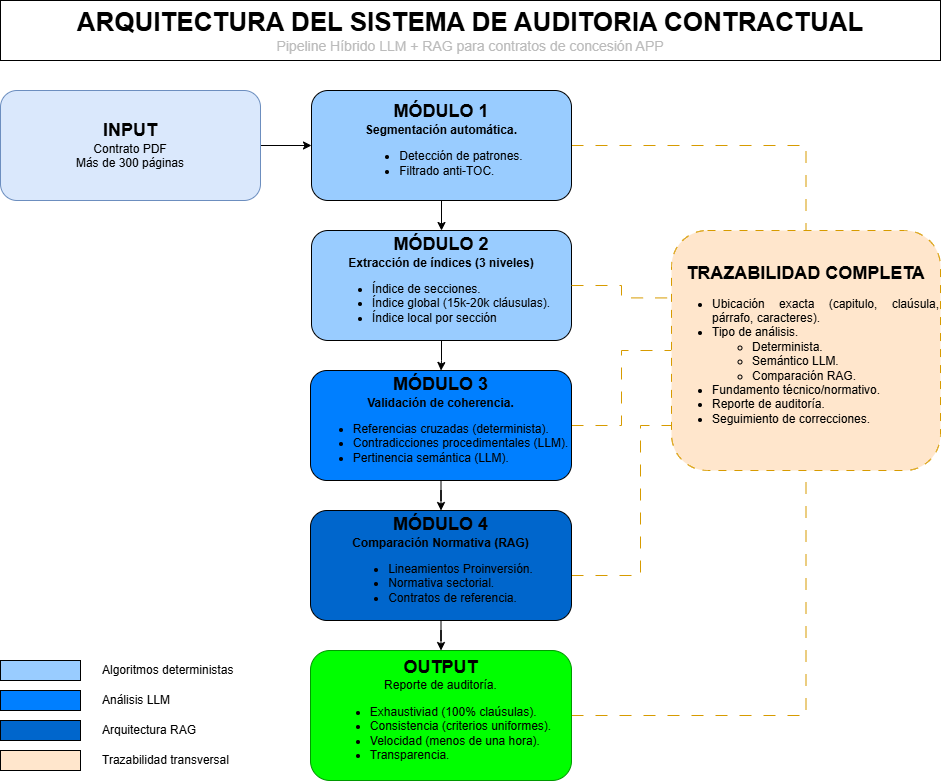
\includegraphics[width=1\linewidth]{images/Diagrama Arquitectura.png}
    \caption{Diagrama de Arquitectura}
    \label{fig:Diagrama de Arquitectura}
\end{figure}

\section{Descripción de Módulos}

\subsection{Input: Contrato PDF}

\begin{tcolorbox}[colback=lightblue!10, colframe=lightblue!80!black, title=Características del Input]
\begin{itemize}[leftmargin=*]
    \item \textbf{Formato:} PDF de contratos de concesión APP
    \item \textbf{Extensión:} Más de 300 páginas
    \item \textbf{Complejidad:} Estructura jerárquica con múltiples niveles
    \item \textbf{Contenido:} Cláusulas contractuales, anexos, referencias normativas
\end{itemize}
\end{tcolorbox}

El sistema recibe como entrada contratos en formato PDF que requieren preprocesamiento para extraer texto, mantener estructura y garantizar calidad de datos para análisis posteriores.

\subsection{Módulo 1: Segmentación Automática}

\begin{tcolorbox}[colback=lightblue!20, colframe=lightblue!80!black, title=Objetivos del Módulo 1]
Dividir el documento en unidades lógicas procesables mientras se elimina contenido no relevante como tablas de contenido (TOC).
\end{tcolorbox}

\subsubsection{Componentes}

\begin{enumerate}[leftmargin=*]
    \item \textbf{Detección de patrones:}
    \begin{itemize}
        \item Identificación de marcadores estructurales (capítulos, secciones, cláusulas)
        \item Reconocimiento de jerarquía mediante numeración y formato
        \item Análisis de encabezados y separadores
    \end{itemize}
    
    \item \textbf{Filtrado anti-TOC:}
    \begin{itemize}
        \item Eliminación de índices y tablas de contenido
        \item Detección de páginas introductorias no contractuales
        \item Limpieza de metadatos y elementos de navegación
    \end{itemize}
\end{enumerate}

\subsubsection{Salida}

Documento segmentado en bloques estructurados listos para indexación, con eliminación de contenido redundante o no relevante.

\subsection{Módulo 2: Extracción de Índices (3 niveles)}

\begin{tcolorbox}[colback=lightblue!20, colframe=lightblue!80!black, title=Objetivos del Módulo 2]
Generar índices jerárquicos que permitan navegación eficiente y extracción selectiva de información en diferentes niveles de granularidad.
\end{tcolorbox}

\subsubsection{Niveles de Indexación}

\begin{enumerate}[leftmargin=*]
    \item \textbf{Índice de secciones:}
    \begin{itemize}
        \item Estructura de alto nivel del contrato
        \item Identificación de capítulos principales
        \item Mapeo de organización general del documento
    \end{itemize}
    
    \item \textbf{Índice global (15\%-20\% de cláusulas):}
    \begin{itemize}
        \item Selección de cláusulas más relevantes
        \item Cobertura estratégica del contenido contractual
        \item Optimización para búsquedas frecuentes
    \end{itemize}
    
    \item \textbf{Índice focal por sección:}
    \begin{itemize}
        \item Granularidad máxima dentro de cada sección
        \item Acceso directo a cláusulas específicas
        \item Contexto local preservado
    \end{itemize}
\end{enumerate}

\subsubsection{Beneficios}

\begin{itemize}[leftmargin=*]
    \item Búsqueda eficiente en documentos extensos
    \item Reducción de tiempo de procesamiento
    \item Mantenimiento de contexto jerárquico
    \item Base para trazabilidad precisa
\end{itemize}

\subsection{Módulo 3: Validación de Coherencia}

\begin{tcolorbox}[colback=mediumblue!20, colframe=mediumblue!80!black, title=Objetivos del Módulo 3]
Verificar la consistencia interna del contrato mediante tres enfoques complementarios: análisis determinista, detección de contradicciones procedimentales y validación semántica.
\end{tcolorbox}

\subsubsection{Enfoques de Validación}

\begin{enumerate}[leftmargin=*]
    \item \textbf{Referencias cruzadas (Determinista):}
    \begin{itemize}
        \item Verificación de referencias internas (e.g., "según cláusula 3.2")
        \item Validación de existencia de cláusulas referenciadas
        \item Detección de referencias rotas o circulares
        \item Algoritmos basados en reglas y expresiones regulares
    \end{itemize}
    
    \item \textbf{Contradicciones procedimentales (LLM):}
    \begin{itemize}
        \item Identificación de cláusulas con información contradictoria
        \item Análisis de plazos, montos y obligaciones inconsistentes
        \item Detección de conflictos entre términos generales y específicos
        \item Uso de modelos de lenguaje para comprensión contextual
    \end{itemize}
    
    \item \textbf{Pertinencia semántica (LLM):}
    \begin{itemize}
        \item Evaluación de coherencia temática entre secciones
        \item Verificación de alineación con objetivos contractuales
        \item Detección de cláusulas fuera de contexto
        \item Análisis de consistencia terminológica
    \end{itemize}
\end{enumerate}

\subsubsection{Tecnología}

\begin{itemize}[leftmargin=*]
    \item \textbf{Algoritmos deterministas:} Expresiones regulares, análisis sintáctico
    \item \textbf{LLM:} Modelos de lenguaje fine-tuned para análisis contractual
    \item \textbf{Validación híbrida:} Combinación de precisión determinista y comprensión semántica
\end{itemize}

\subsection{Módulo 4: Comparación Normativa (RAG)}

\begin{tcolorbox}[colback=darkblue!20, colframe=darkblue!80!black, title=Objetivos del Módulo 4]
Comparar el contrato contra documentos normativos y contratos de referencia utilizando arquitectura RAG para garantizar cumplimiento regulatorio y mejores prácticas.
\end{tcolorbox}

\subsubsection{Bases de Conocimiento}

\begin{enumerate}[leftmargin=*]
    \item \textbf{Lineamientos Proinversión:}
    \begin{itemize}
        \item Guías oficiales para contratos de concesión APP
        \item Estándares de estructuración contractual
        \item Requisitos mínimos obligatorios
    \end{itemize}
    
    \item \textbf{Normativa sectorial:}
    \begin{itemize}
        \item Leyes y reglamentos aplicables
        \item Resoluciones ministeriales específicas
        \item Jurisprudencia relevante
    \end{itemize}
    
    \item \textbf{Contratos de referencia:}
    \begin{itemize}
        \item Contratos similares previamente aprobados
        \item Mejores prácticas documentadas
        \item Casos de éxito y lecciones aprendidas
    \end{itemize}
\end{enumerate}

\subsubsection{Arquitectura RAG}

\begin{itemize}[leftmargin=*]
    \item \textbf{Retrieval:} Búsqueda semántica en bases documentales
    \item \textbf{Augmentation:} Enriquecimiento del contexto con información normativa
    \item \textbf{Generation:} Generación de hallazgos con fundamento regulatorio
\end{itemize}

\subsubsection{Proceso}

\begin{enumerate}[leftmargin=*]
    \item Extracción de cláusulas del contrato analizado
    \item Búsqueda de secciones normativas relevantes
    \item Comparación semántica entre contrato y normativa
    \item Identificación de desviaciones o cumplimiento
    \item Generación de recomendaciones fundamentadas
\end{enumerate}

\subsection{Output: Reporte de Auditoría}

\begin{tcolorbox}[colback=lightgreen!20, colframe=lightgreen!80!black, title=Características del Reporte]
El sistema genera un reporte exhaustivo con cuatro atributos clave que garantizan su utilidad y confiabilidad.
\end{tcolorbox}

\subsubsection{Atributos del Reporte}

\begin{enumerate}[leftmargin=*]
    \item \textbf{Exhaustividad (100\% de cláusulas):}
    \begin{itemize}
        \item Cobertura completa del contrato
        \item Ninguna cláusula queda sin analizar
        \item Métricas de cobertura documentadas
    \end{itemize}
    
    \item \textbf{Consistencia (criterios uniformes):}
    \begin{itemize}
        \item Aplicación homogénea de criterios de auditoría
        \item Eliminación de sesgos subjetivos
        \item Comparabilidad entre diferentes contratos
    \end{itemize}
    
    \item \textbf{Velocidad (menos de una hora):}
    \begin{itemize}
        \item Procesamiento automatizado de alto rendimiento
        \item Reducción drástica vs. auditoría manual (semanas)
        \item Escalabilidad para múltiples contratos
    \end{itemize}
    
    \item \textbf{Transparencia:}
    \begin{itemize}
        \item Trazabilidad completa de cada hallazgo
        \item Justificación técnica y normativa explícita
        \item Reproducibilidad de resultados
    \end{itemize}
\end{enumerate}

\subsubsection{Estructura del Reporte}

\begin{itemize}[leftmargin=*]
    \item Resumen ejecutivo
    \item Hallazgos por categoría (coherencia, normativa)
    \item Nivel de criticidad (alto, medio, bajo)
    \item Recomendaciones específicas
    \item Anexos con trazabilidad detallada
\end{itemize}

\section{Trazabilidad Completa}

\begin{tcolorbox}[colback=lightorange!20, colframe=orange!80!black, title=Sistema de Trazabilidad Transversal]
La trazabilidad es un componente fundamental que atraviesa todos los módulos del sistema, garantizando que cada hallazgo pueda ser verificado y auditado.
\end{tcolorbox}

\subsection{Componentes de la Trazabilidad}

\subsubsection{Ubicación Exacta}

Para cada hallazgo, el sistema registra:

\begin{itemize}[leftmargin=*]
    \item \textbf{Capítulo:} Sección principal del contrato
    \item \textbf{Cláusula:} Numeración específica de la cláusula
    \item \textbf{Párrafo:} Ubicación dentro de la cláusula
    \item \textbf{Caracteres:} Rango exacto de caracteres en el texto original
\end{itemize}

Esta granularidad permite:
\begin{itemize}
    \item Localización inmediata en el documento fuente
    \item Verificación manual cuando sea necesario
    \item Generación de hipervínculos directos
\end{itemize}

\subsubsection{Tipo de Análisis}

Cada hallazgo se clasifica según el método que lo identificó:

\begin{enumerate}[leftmargin=*]
    \item \textbf{Determinista:}
    \begin{itemize}
        \item Basado en reglas algorítmicas
        \item Alta precisión y reproducibilidad
        \item Ejemplos: referencias rotas, formato incorrecto
    \end{itemize}
    
    \item \textbf{Semántico LLM:}
    \begin{itemize}
        \item Análisis mediante modelos de lenguaje
        \item Comprensión contextual profunda
        \item Ejemplos: contradicciones, pertinencia
    \end{itemize}
    
    \item \textbf{Comparación RAG:}
    \begin{itemize}
        \item Contraste con documentación externa
        \item Fundamentación normativa
        \item Ejemplos: incumplimientos regulatorios, desviaciones de estándares
    \end{itemize}
\end{enumerate}

\subsubsection{Fundamento Técnico/Normativo}

Cada hallazgo incluye:

\begin{itemize}[leftmargin=*]
    \item \textbf{Base técnica:} Explicación del problema identificado
    \item \textbf{Referencia normativa:} Ley, artículo o lineamiento aplicable
    \item \textbf{Severidad:} Evaluación del impacto (crítico, alto, medio, bajo)
    \item \textbf{Recomendación:} Acción correctiva sugerida
\end{itemize}

\subsubsection{Reporte de Auditoría}

El reporte integra toda la información trazable en un formato accesible:

\begin{itemize}[leftmargin=*]
    \item Resumen de hallazgos con enlaces a ubicaciones exactas
    \item Clasificación por tipo y severidad
    \item Gráficos de distribución de hallazgos
    \item Matriz de cumplimiento normativo
\end{itemize}

\subsubsection{Seguimiento de Correcciones}

El sistema permite:

\begin{itemize}[leftmargin=*]
    \item Marcar hallazgos como resueltos
    \item Adjuntar evidencia de corrección
    \item Re-analizar secciones modificadas
    \item Mantener historial de versiones
\end{itemize}

\subsection{Beneficios de la Trazabilidad}

\begin{enumerate}[leftmargin=*]
    \item \textbf{Auditoría externa:} Facilita la verificación por terceros
    \item \textbf{Aprendizaje continuo:} Permite mejorar algoritmos mediante feedback
    \item \textbf{Cumplimiento regulatorio:} Demuestra debida diligencia
    \item \textbf{Gestión de riesgos:} Priorización basada en evidencia
    \item \textbf{Transparencia:} Genera confianza en stakeholders
\end{enumerate}

\section{Conclusiones}

El Sistema de Auditoría Contractual representa una solución innovadora que combina lo mejor de tres mundos:

\begin{itemize}[leftmargin=*]
    \item \textbf{Algoritmos deterministas} para precisión y reproducibilidad
    \item \textbf{Large Language Models} para comprensión semántica profunda
    \item \textbf{Arquitecturas RAG} para fundamentación normativa actualizada
\end{itemize}

La arquitectura modular permite evolución independiente de componentes, mientras que el sistema de trazabilidad transversal garantiza auditabilidad y transparencia en cada hallazgo. El resultado es una herramienta que no solo automatiza la auditoría contractual, sino que la eleva a un nuevo estándar de calidad, velocidad y confiabilidad.

\end{document}